\documentclass{article}
\usepackage[T1]{fontenc}
\usepackage{amssymb}
\usepackage{hyperref}
\usepackage{amsmath}
\usepackage{xcolor}
\usepackage{listings}
\usepackage{graphicx}


\definecolor{mGreen}{rgb}{0,0.6,0}
\definecolor{mGray}{rgb}{0.5,0.5,0.5}
\definecolor{mPurple}{rgb}{0.58,0,0.82}
\definecolor{backgroundColour}{RGB}{206, 206, 206}

\lstdefinestyle{CStyle}{
    backgroundcolor=\color{backgroundColour},   
    commentstyle=\color{mGreen},
    keywordstyle=\color{magenta},
    numberstyle=\tiny\color{mGray},
    stringstyle=\color{mPurple},
    basicstyle=\footnotesize,
    breakatwhitespace=false,         
    breaklines=true,                 
    captionpos=b,                    
    keepspaces=true,                 
    numbers=left,                    
    numbersep=5pt,                  
    showspaces=false,                
    showstringspaces=false,
    showtabs=false,                  
    tabsize=2,
    language=C
}
\hypersetup{
    colorlinks,
    citecolor=black,
    filecolor=black,
    linkcolor=black,
    urlcolor=black
}

\title{PWRinSPACE\\Symulator silnika na paliwo stałe dla geometrii BYTES}
\author{Manfred Gawlas}
\date{29.11.2023}

\begin{document}
\maketitle
\begin{abstract}
Dokument ten przedstawia ręcznie napisany symulator silnika na paliwo stałe dla różnych typów pochodnych od geometrii BYTES, algortym wykonujący symulacje oraz prezentuje wzory fizyczne potrzebne do przeprowadzenia takiej symulacji.
    \end{abstract}
\section{Input}
\begin{itemize}
\item Dane dla konkretnego paliwa: $\rho_p, T_0, k, R_s, a, n$
\item Burn rate coefficient $a$
\item Pressure exponent $n$
\item Funkcje Area burning $A_b(t, r)$
\item Początkowe ciśnienie w komorze $P_0$
\item Rozmiary komory oraz rdzenia$L, D, d$
\item Ciąg początkowy przed poprawką $F_{pocz}$
\end{itemize}

\section{Output}
\begin{itemize}
\item Ciąg $F$
\item Wymiary dyszy: $A_t, A_e$
\item Czas spalania $t$
\item Impuls całkowity $I_t$
\end{itemize}

\section{Wzory}
Wszystkie potrzebne w tym symulatorze wzory pochodzą z "Rocketry formulas and derivations" autorstwa Sebastiana Króla(BAZA).\\\\
\textbf{1)} Pierwszym ważnym wzorem którego będziemy używać jest wzór na ciąg silniku.
\begin{equation} F=A_tP_0\sqrt{\frac{2k^2}{k-1}\left(\frac{2}{k+1}\right)^{\frac{k+1}{k-1}}\left[1-\left(\frac{P_e}{P_0}\right)^{\frac{k-1}{k}}\right]} \end{equation}
Zakładając $C_F$ równe

\begin{equation} C_F=\sqrt{\frac{2k^2}{k-1}\left(\frac{2}{k+1}\right)^{\frac{k+1}{k-1}}\left[1-\left(\frac{P_e}{P_0}\right)^{\frac{k-1}{k}}\right]} \end{equation}
Otrzymujemy 
\begin{equation} F=A_tP_0C_F\end{equation}
\textbf{2)} Jako że mamy podany ciąg początkowy $F_0$ i zakładamy sobie jakieś ciśnienie początkowe to liczymy dla nich $A_t$. 
\begin{equation} A_t=\frac{F_0}{P_0C_F} \end{equation}
\textbf{3)} Dla $A_e$ obliczamy je z
\begin{equation}A_e=\frac{A_t}{\left(\frac{k+1}{2}\right)^{\frac{1}{k-1}}\left(\frac{P_e}{P_0}\right)^{\frac{1}{k}}\sqrt{\left(\frac{k+1}{k-1}\right)\left[1-\left(\frac{P_e}{P_0}\right)^{\frac{k-1}{k}}\right]}}\end{equation}
\textbf{4)} Ścisły wzór na impuls całkowity
$$Ic=\int^{t_1}_0F(t)dt$$
Całke tą będziemy rozwiązywać metodą graficzną prostokontów, ale dokładniej o tym w sekcji o algorytmie.\\\\
\textbf{5)} Ciśnienie jako funkcja $A_b$:
\begin{equation}P_{ch}(A_b)=K_n^{\frac{1}{1-n}}(c^*\rho_pa)^{\frac{1}{1-n}}\end{equation}
Co wyprowadzamy z wzorów:
$$r=ap^n$$
$$\dot{m}=r\rho_pA_b$$
$$c^*=\frac{A_tP_{ch}}{\dot{m}}$$

\section{Geometria ziarna}
Projekt ten będzie brał pod uwagę tylko geometrie typu BYTES, jako że inne zdają sie albo nie spełniać wymagać albo są ciężkie do policzenia. Geometrie typu BYTES można zaposać w ogólnej postaci:
$$A_b(t)=A_w(t)+kA_z(t)$$
gdzie k to liczba powierzchni bocznych walca które ulegają spalaniu. Dla 1 walcowego modelu jest to liczba z przedziału $k\in\{0, 1, 2\}$. Dla geometrii bytes z wieloma walcami dochodzą nam dodatkowe powierzchnie.
$$A_w(t)=2\pi R(t)L(t)$$
gdzie  $A_w$ powierzchnia spalania wewnętrzna(zewnętrzna rdzenia), R promień rdzenia, L suma długość rdzeni. 
$$A_z(t)=\pi \frac{D^2}{4} - \pi R^2(t)$$
gdzie $A_z$ powierzchnia spalania na jednej podstawie walca, D średnica komory spalania, R promień rdzenia. To jest zakładając że rdzenie wszystkich rdzeni jest tożsamy.\\\\
Funckcje $L(t)$ oraz $R(t)$ wyrażają sie wzorami, lub przez ciągi rekurencyjne:
$$L(t)=L_0 - kr(P_0)t$$
$$L_n=L_{n-1} - kr_n\Delta t$$
$$R(t)=\frac{d}{2} + r(P_0)t$$
$$R_n=R_{n-1}+r_n\Delta t$$
\section{Algorytm}
W tej sekcji przedstawie po krótce jak działa główny algorytm symulatora silniku. Jest on częściowo tożsamy z algorytmem liczącym całke oznaczoną metodą prostokątków. Impuls całkowiny jest liczony właśnie całką dla czasu $\Delta t$ oraz ciągu chwilowego $F_0$.
$$Ic\approx \sum^n_{i=0}F_i\Delta t$$
Gdzie  $\Delta t$ to dowolny mały okres czasu dla którego przyjmujemy $P_0=const$, $r=const$. Co za tym idzie zakładamy $F_i=const$ dla tego okresu. Kolejne $F_i$ będą wyznaczane podczas działania algorytmu.\\\\
Pierwszym krokiem jest policznenie poprawki dla założonego ciśnienia i ciągu początkowego. Kożystamy wiec z równania (4) i wyznaczamy $A_t$. Następnie przy pomocy wzoru (6) na $P_ch$ wyznaczamy rzeczywiste ciśnienie.  Po policzeniu poprawki możemy zacząć główną pętle programu.

\subsection*{Warunek pętli}
Pętla wykonuje się dopuki nie spali się cale paliwo, a więc dopuki zmienna $$\mbox{totalRegressed} < \frac{D-d}{2}$$

\subsection*{Krok 1}
Liczymy chwilowy ciąg silnika oraz następnie dodajemy jego iloczyn(całka metodą prostokątu) do impulsu.
$$F=A_tP_0C_F$$
$$Ic+=F\Delta t$$

\subsection*{Krok 2}
Liczymy chwilową regresje dla tego okresu czasu:
$$r=aP_0^n$$

\subsection*{Krok 3}
Z pomocą obliczonej regresji obliczamy jaka zmiana zaszła dla wartości $A_b$
$$R=R+r\Delta t$$
$$L=L - kr\Delta t$$
\subsection*{Krok 4} 
Obliczamy nową wartość $P_0$ za pomocą wzoru (6)
$$P_0(A_b)=K_n^{\frac{1}{1-n}}(c^*\rho_pa)^{\frac{1}{1-n}}$$
\subsection*{Krok 5}
Aktualizujemy zmienną totalRegressed.
$$\mbox{totalRegressed} +=\Delta t r$$
\newpage
\section{Symulator}
W pierwszej części tej sekcji umieszcze jego implementacje w C, a w drugiej przedstawie porównanie dla modelu 32x120 mm, $d=20mm$, zakładane ciśnienie $P_0=30atm$, w geometrii BYTES, z 1 powierzchnią podstawy palenia, pomiędzy moim symulatorem a programem openRocket.
\subsection*{Implementacja w C}

\begin{lstlisting}[style=CStyle]
// ster.c Manfred Gawlas

#include <stdio.h>
#include <math.h>

struct AbGeometry // Grain size
{
	double L;
	double R;
	double D;
};

struct General // General variables that we often use
{
	double Pch;
	double L;
	double D;
	double d;
	double At;
	double Pe;
};

struct Fuel // Size of grain
{
	double Cstar;
	double a;
	double n;
	double k;
	double rho;
};

double CF(struct General Cylinder, struct Fuel RNX71) // Function that returns value of CF
{
	return pow((2*RNX71.k*RNX71.k)/(RNX71.k-1) * pow(2/(RNX71.k+1), (RNX71.k+1)/(RNX71.k-1)) * (1 - pow(Cylinder.Pe/Cylinder.Pch, (RNX71.k-1)/RNX71.k)), 0.5);
}

double F(struct General Cylinder, struct Fuel RNX71) // Function that returns thursh value
{
	return CF(Cylinder, RNX71) * Cylinder.At * Cylinder.Pch;
}

double FunctionAb(struct AbGeometry Ab) // Function that returns area burning
{
	return 3.14159*(2*Ab.L*Ab.R + 0.25*Ab.D*Ab.D - Ab.R*Ab.R);
}


int main(void)
{
	// All values are in basic SI units

	double r=0;
	double Ic=0;
	double F0=82.37528;
	double tc=0;
	double totalRegressed=0; // Stores how deap it burned in
	double Deltat=0.003; // Time period for which our loop works

	struct General Cylinder;
	Cylinder.Pch=30*101325; 
	Cylinder.L=0.12;
	Cylinder.D=0.032;
	Cylinder.d=0.020;
	//Cylinder.At=0.00001824875;
	Cylinder.Pe=101325;
	
	struct Fuel RNX71;
	RNX71.Cstar=779;
	RNX71.a=0.0000163938; // Counted by hand from a for MPa, this one is for Pa
	RNX71.n=0.371;
	RNX71.k=1.18;
	RNX71.rho=1848;

	struct AbGeometry Ab;
	Ab.L=Cylinder.L;
	Ab.R=Cylinder.d/2;
	Ab.D=Cylinder.D;
	
	//printf("F0=%f\n", F(Cylinder, RNX71));
	//printf("CF=%f\n\n", CF(Cylinder, RNX71));
	

	Cylinder.At=F0/(Cylinder.Pch*CF(Cylinder, RNX71));
	Cylinder.Pch=pow(FunctionAb(Ab) / Cylinder.At, 1/(1-RNX71.n)) * pow(RNX71.Cstar * RNX71.rho * RNX71.a, 1/(1-RNX71.n));
	

	//////////////////////////////////
	// Main loop, algorithm similar to calculating integrad by rectangles.
	//////////////////////////////////
	
	while(totalRegressed<((Cylinder.D-Cylinder.d)/2))
	{
		//  Value of time, thrust and updating value of impuls

		tc+=Deltat;
		F0=F(Cylinder, RNX71);
		Ic+=F0 * Deltat;
		
		
		///////////////////////////////
		// You can print values for any variable. Helps with making graphs.
		///////////////////////////////
		
		printf("%f\n", F0);
		//printf("%f\n\n", Ic);
		//printf("%f\n", FunctionAb(Ab)/Cylinder.At); // Kn
		//printf("%f\n", Cylinder.Pch);
		
		///////////////////////////////

		r=RNX71.a * pow(Cylinder.Pch, RNX71.n);
		Ab.L=Ab.L - r*Deltat;
		Ab.R=Ab.R + r*Deltat;

		Cylinder.Pch=pow(FunctionAb(Ab) / Cylinder.At, 1/(1-RNX71.n)) * pow(RNX71.Cstar * RNX71.rho * RNX71.a, 1/(1-RNX71.n));
		
		totalRegressed+=r*Deltat; // Updates how much already burned
	}


	// Print of end values
	
	printf("Ic=%f\n", Ic);
	printf("tc=%f\n", tc);	
	printf("Pch=%f\n", Cylinder.Pch);	

	return 0;
}
\end{lstlisting}
\newpage
\subsection*{Porównanie symulatorów}
Wykresy $K_n$.\\ Wykres 1 mój symulator:\\
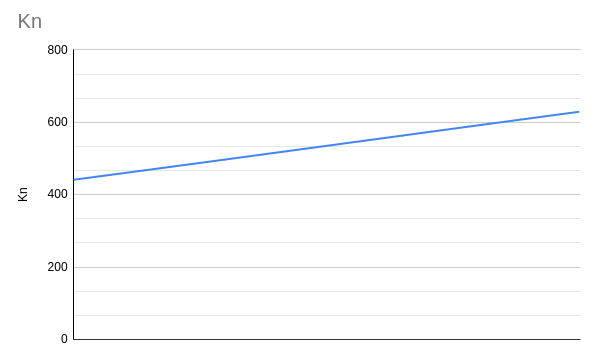
\includegraphics[width=11cm]{moje1}\\
Wykres 2 openMotor:\\
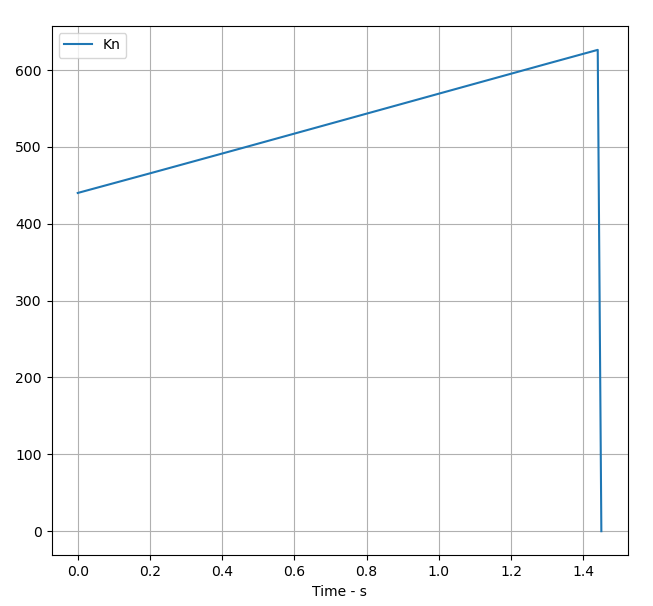
\includegraphics[width=11cm]{openMotor1}\\\\
Wykresy ciągu.\\ Wykres 1 mój symulator:\\
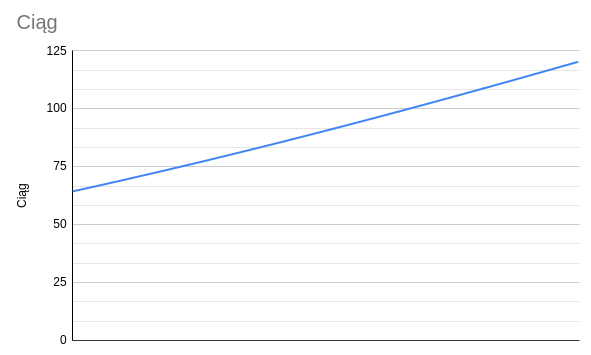
\includegraphics[width=11cm]{moje2}\\
Wykres 2 openMotor:\\
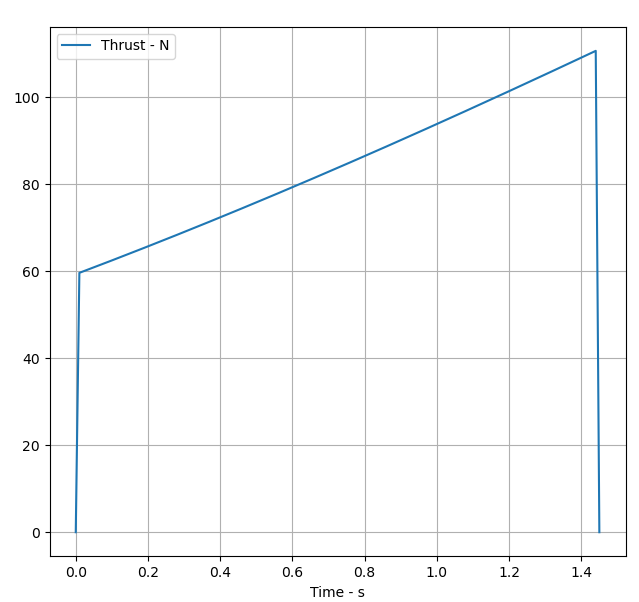
\includegraphics[width=11cm]{openMotor2}\\\\\\
Podsumowując, symulatory zwracają bardzo podobne wyniki, gdzie błąd jest spowodowany w dużym stopniu przez różne przybliżenia dla niektórych parametrów. Np. fakt że do openMotora można wpisać współczynnik regresji tylko dla 2 miejsc znaczących, generuje 4\% błędu na ciśnieniu itd. Wiadomo że dane te są i tak niedokładne, więc te kilku procentowe błędy ostatecznie raczej nie są do końca możliwe do pozbycia się w sensownym stopniu.



\end{document}